\section{biguint-cmp}
\label{biguint-cmp}

\begin{enumerate}
    \item target
        \begin{itemize}
            \item implement the comparison of two biguints
        \end{itemize}
    \item constraints-logic
        \begin{itemize}
            \item split the input to many limbs, such that: limbs-num = bits / chunks
            \item execute comparison for low bits limbs
            \item ensure that the result is determined by the highest limbs which are not equal
        \end{itemize}
    \item biguint-cmp process layout
        \begin{figure}[!ht]
            \centering
            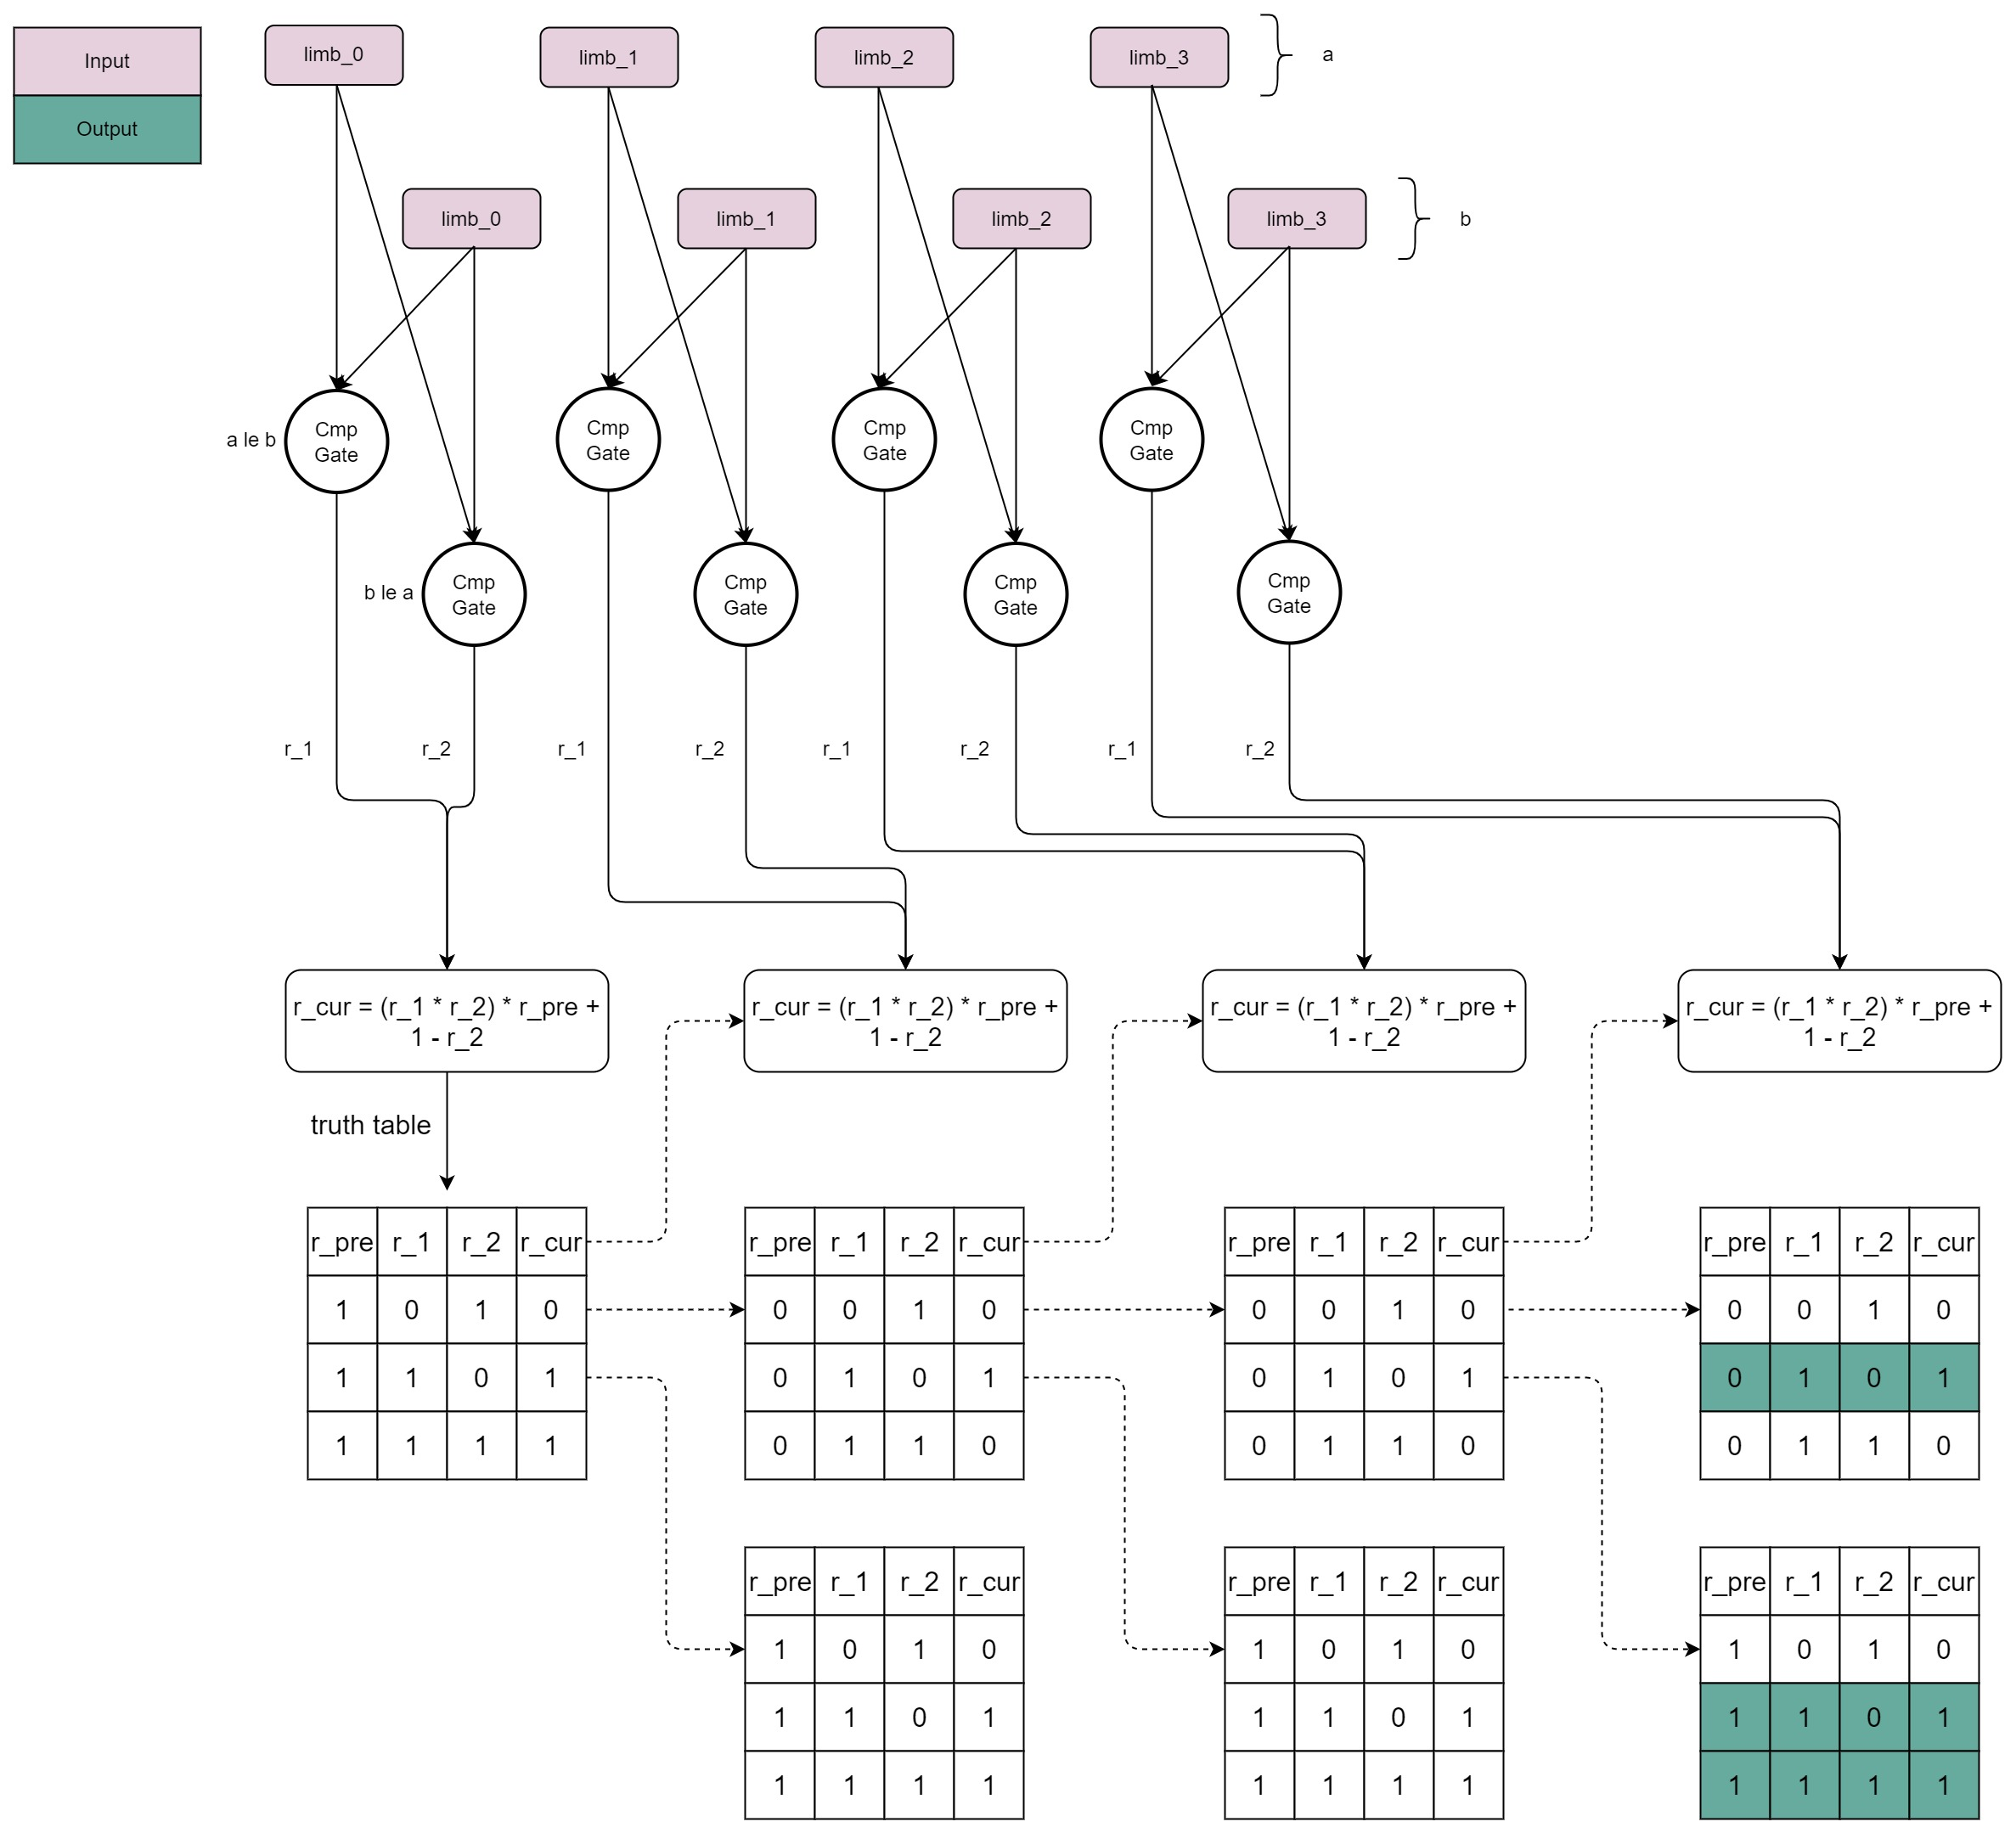
\includegraphics[width=0.8\textwidth]{biguint-cmp-layout.jpg}
            \caption{biguint-cmp layout.jpg}
            \label{fig:biguint-cmp-layout.jpg}
        \end{figure}
    \item biguint-cmp circuit layout
    \begin{figure}[!ht]
        \centering
        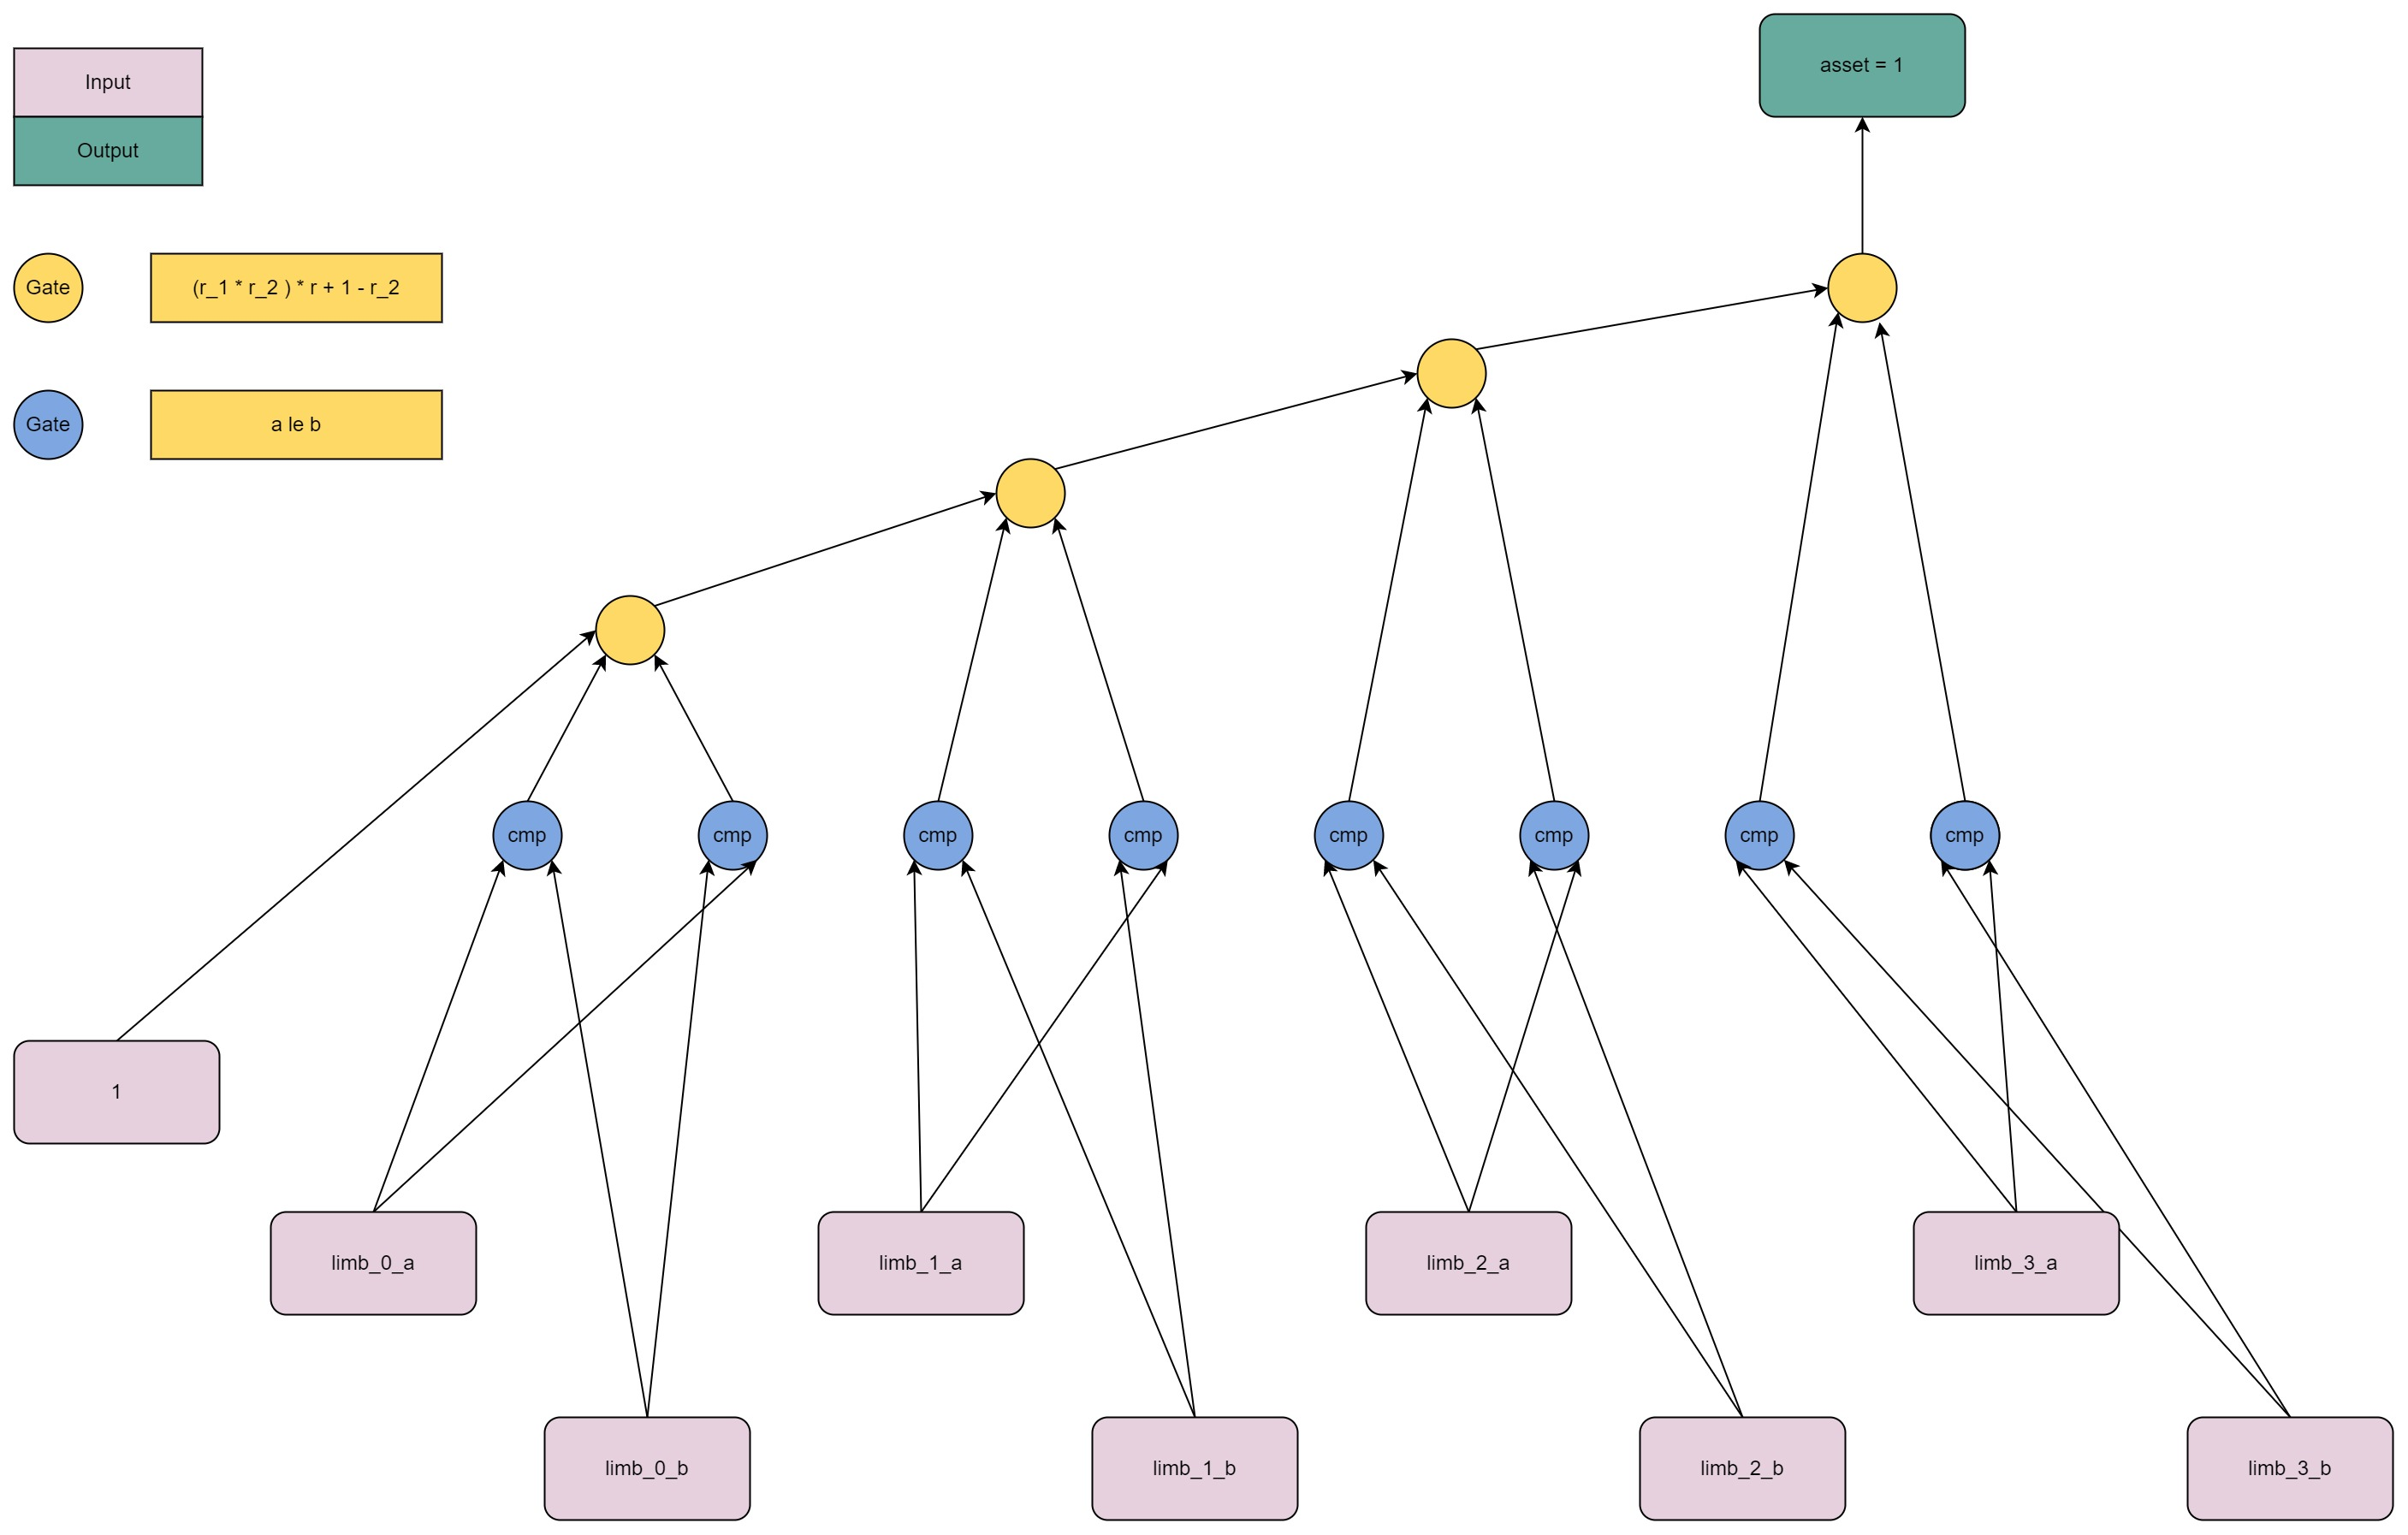
\includegraphics[width=0.8\textwidth]{biguint-cmp-circuit-layout.jpg}
        \caption{biguint-cmp circuit layout.jpg}
        \label{fig:biguint-cmp-circuit-layout.jpg}
    \end{figure}
    
    \item constraints-info and costs
        \begin{itemize}
            \item Gate type num: 2(ComparisionGate, ArithmeticGate)
            \item Gate instance num: 4 * 2 + 3 = 11 
            \item ComparisionGate num: 8
            \item ArithmeticGate num: 3
            \item copy-constraints: (4 + 9) * 4 + 1 = 53 
            \item max-degree: 4
        \end{itemize}

\end{enumerate}